%package list
\documentclass{article}
\usepackage[top=3cm, bottom=3cm, outer=3cm, inner=3cm]{geometry}
\usepackage{multicol}
\usepackage{graphicx}
\usepackage{url}
\usepackage{hyperref}
\usepackage{array}
\newcolumntype{x}[1]{>{\centering\arraybackslash\hspace{0pt}}p{#1}}
\usepackage{natbib}
\usepackage{pdfpages}
\usepackage{multirow}
\usepackage[normalem]{ulem}
\useunder{\uline}{\ul}{}
\usepackage{svg}
\usepackage{xcolor}
\usepackage{listings}
\lstdefinestyle{ascii-tree}{
    literate={├}{|}1 {─}{--}1 {└}{+}1 
  }
\lstset{basicstyle=\ttfamily,
  showstringspaces=false,
  commentstyle=\color{red},
  keywordstyle=\color{blue}
}
%\usepackage{booktabs}
\usepackage{caption}
\usepackage{subcaption}
\usepackage{float}
\usepackage{array}

% Comment
\usepackage{verbatim}

\newcolumntype{M}[1]{>{\centering\arraybackslash}m{#1}}
\newcolumntype{N}{@{}m{0pt}@{}}


%%%%%%%%%%%%%%%%%%%%%%%%%%%%%%%%%%%%%%%%%%%%%%%%%%%%%%%%%%%%%%%%%%%%%%%%%%%%
%%%%%%%%%%%%%%%%%%%%%%%%%%%%%%%%%%%%%%%%%%%%%%%%%%%%%%%%%%%%%%%%%%%%%%%%%%%%
\newcommand{\itemEmail}{rzapata@unsa.edu.pe}
\newcommand{\itemStudent}{Reyser Julio Zapata Butrón}
\newcommand{\itemCourse}{Análisis Y Diseño de Algoritmos}
\newcommand{\itemCourseCode}{1702231}
\newcommand{\itemSemester}{IV}
\newcommand{\itemUniversity}{Universidad Nacional de San Agustín de Arequipa}
\newcommand{\itemFaculty}{Facultad de Ingeniería de Producción y Servicios}
\newcommand{\itemDepartment}{Departamento Académico de Ingeniería de Sistemas e Informática}
\newcommand{\itemSchool}{Escuela Profesional de Ingeniería de Sistemas}
\newcommand{\itemAcademic}{2024 - B}
\newcommand{\itemInput}{17 septiembre 2024}
\newcommand{\itemOutput}{17 septiembre 2024}
\newcommand{\itemPracticeNumber}{01}
\newcommand{\itemTheme}{Introducción}
\newcommand{\itemPracticeDuration}{02 horas}
%%%%%%%%%%%%%%%%%%%%%%%%%%%%%%%%%%%%%%%%%%%%%%%%%%%%%%%%%%%%%%%%%%%%%%%%%%%%
%%%%%%%%%%%%%%%%%%%%%%%%%%%%%%%%%%%%%%%%%%%%%%%%%%%%%%%%%%%%%%%%%%%%%%%%%%%%

\usepackage[english,spanish]{babel}
\usepackage[utf8]{inputenc}
\AtBeginDocument{\selectlanguage{spanish}}
\renewcommand{\figurename}{Figura}
\renewcommand{\refname}{Referencias}
\renewcommand{\tablename}{Tabla} %esto no funciona cuando se usa babel
\AtBeginDocument{%
	\renewcommand\tablename{Tabla}
}

\usepackage{fancyhdr}
\pagestyle{fancy}
\fancyhf{}
\setlength{\headheight}{30pt}
\renewcommand{\headrulewidth}{1pt}
\renewcommand{\footrulewidth}{1pt}
\fancyhead[L]{\raisebox{-0.2\height}{
\includegraphics[width=3cm]{img/logo_episunsa.png}}}
\fancyhead[C]{\fontsize{7}{7}\selectfont	\itemUniversity \\ \itemFaculty \\ \itemDepartment \\ \itemSchool \\ \textbf{\itemCourse}}
\fancyhead[R]{\raisebox{-0.2\height}{
\includegraphics[width=1.2cm]{img/logo_abet}}}
\fancyfoot[L]{Reyser Julio Zapata Butrón}
\fancyfoot[C]{\itemCourse}
\fancyfoot[R]{Página \thepage}

% Estilos del Código
\usepackage{listings}
\usepackage{color, colortbl}
\definecolor{dkgreen}{rgb}{0,0.6,0}
\definecolor{gray}{rgb}{0.5,0.5,0.5}
\definecolor{codebackground}{rgb}{89, 0.97, 0.90}
\definecolor{tablebackground}{rgb}{0.8, 0, 0}

\lstset{
  language=C++,                  
  basicstyle=\ttfamily\footnotesize,
  keywordstyle=\color{blue},     
  commentstyle=\color{dkgreen},    
  stringstyle=\color{red},       
  backgroundcolor= \color{codebackground},
  numbers=left,                  
  numberstyle=\tiny\color{gray},
  stepnumber=1,                  
  numbersep=5pt,                
  showspaces=false,              
  showstringspaces=false,      
  showtabs=false,                
  frame=single,                  
  captionpos=b,                  %
}

\begin{document}
	\vspace*{10px}
	
	\begin{center}	
		\fontsize{17}{17} \textbf{ Informe de Laboratorio \itemPracticeNumber}
	\end{center}

 %% TABLA %%
 
	\centerline{\textbf{\Large Tema: \itemTheme}}

	\begin{flushright}
		\begin{tabular}{|M{2.5cm}|N|}
			\hline 
			\rowcolor{tablebackground}
			\color{white} \textbf{Nota}  \\
			\hline 
			     \\[30pt]
			\hline 			
		\end{tabular}
	\end{flushright}	

	\begin{table}[H]
		\begin{tabular}{|x{4.7cm}|x{4.8cm}|x{4.8cm}|}
			\hline 
			\rowcolor{tablebackground}
			\color{white} \textbf{Estudiante} & \color{white}\textbf{Escuela}  & \color{white}\textbf{Asignatura}   \\
			\hline 
			{\itemStudent \par \itemEmail} & \itemSchool & {\itemCourse \par Semestre: \itemSemester \par Código: \itemCourseCode}     \\
			\hline 			
		\end{tabular}
	\end{table}		
	
	\begin{table}[H]
		\begin{tabular}{|x{4.7cm}|x{4.8cm}|x{4.8cm}|}
			\hline 
			\rowcolor{tablebackground}
			\color{white}\textbf{Laboratorio} & \color{white}\textbf{Tema}  & \color{white}\textbf{Duración}   \\
			\hline 
			\itemPracticeNumber & \itemTheme & \itemPracticeDuration   \\
			\hline 
		\end{tabular}
	\end{table}
	
	\begin{table}[H]
		\begin{tabular}{|x{4.7cm}|x{4.8cm}|x{4.8cm}|}
			\hline 
			\rowcolor{tablebackground}
			\color{white}\textbf{Semestre académico} & \color{white}\textbf{Fecha de inicio}  & \color{white}\textbf{Fecha de entrega}   \\
			\hline 
			\itemAcademic & \itemInput &  \itemOutput  \\
			\hline 
		\end{tabular}
	\end{table}

 %% CONTENIDO %%
\section{Ejercicios}
Se eligieron los ejercicios 2, 4, 7, 9 y 10 para el informe actual, sin embargo se realizaron los 10 ejercicios y se encuentran en el repositorio de Github. \\

En la mayoría de los ejercicios, se utilizaron argumentos en línea de comandos para proporcionar datos de entrada al programa de manera eficiente. Además, se emplearon arrays dinámicos para manejar datos de tamaño variable y optimizar el uso de memoria.

    \subsection{Ejercicio 2}
        \begin{itemize}
            \item Desarrollar un programa que tenga como entrada un array de números y muestre en la salida
            los números con la respectiva posición que ocupa en el array.
        \end{itemize}  
        
        \lstinputlisting[language=C++, caption={ejercicio2.cpp}, numbers=left]{src/ejercicio2.cpp}

        \textbf{Ejecución del ejercicio}
        \begin{figure}[H]
        	\centering
         	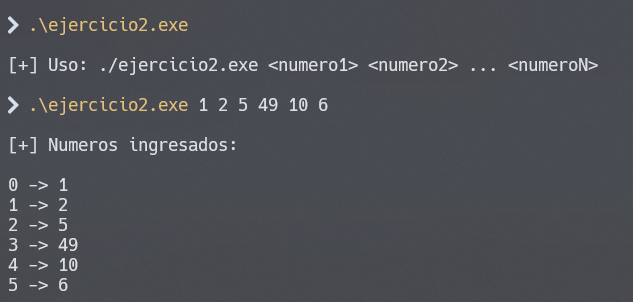
\includegraphics[width=0.8\textwidth,keepaspectratio]{img/ejercicio2.png}
        \end{figure}
        
    
    \subsection{Ejercicio 4}
        \begin{itemize}
            \item Desarrollar un programa que lea la entrada estándar un array de enteros y determine el
            menor elemento del array.
        \end{itemize}
    
        \lstinputlisting[language=C++, caption={ejercicio4.cpp}, numbers=left]{src/ejercicio4.cpp}

        \textbf{Ejecución del ejercicio}
        \begin{figure}[H]
        	\centering
         	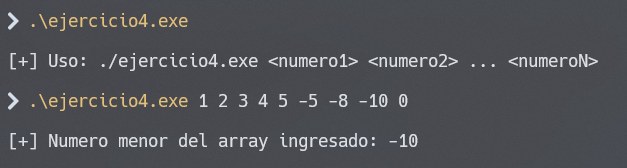
\includegraphics[width=0.8\textwidth,keepaspectratio]{img/ejercicio4.png}
        \end{figure}

    
    \subsection{Ejercicio 7}
        \begin{itemize}
            \item Crear un programa que lea 10 elementos en un array, los copie a otro array multiplicado por
            un número que se ingrese por teclado. Mostrar el contenido del nuevo array.
        \end{itemize}
        
        \lstinputlisting[language=C++, caption={ejercicio7.cpp}, numbers=left]{src/ejercicio7.cpp}

        \textbf{Ejecución del ejercicio}
        \begin{figure}[H]
        	\centering
         	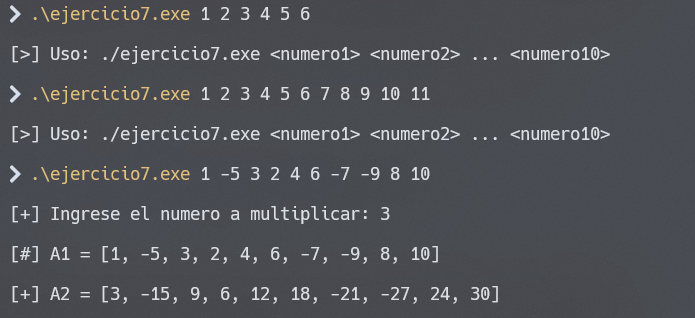
\includegraphics[width=0.8\textwidth,keepaspectratio]{img/ejercicio7.png}
        \end{figure}
        
    
    \subsection{Ejercicio 9}
        \begin{itemize}
            \item Dada un array de enteros, mueva todos los ceros presentes al final del array. La solución
            debe mantener el orden relativo de los elementos en el array y no debe usar un espacio constante.
        \end{itemize}
        
        \lstinputlisting[language=C++, caption={ejercicio9.cpp}, numbers=left]{src/ejercicio9.cpp}
        
        \textbf{Ejecución del ejercicio}
        \begin{figure}[H]
        	\centering
         	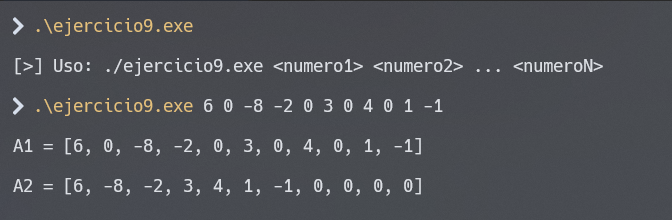
\includegraphics[width=0.8\textwidth,keepaspectratio]{img/ejercicio9.png}
        \end{figure}
        
    
    \subsection{Ejercicio 10}
        \begin{itemize}
            \item Desarrollar un programa que permita ingresar varios números. Almacene los números pares en
            un array llamado numPar[] y los números impares en un array llamado numImpar[]. Finalmente
            deberá mostrar los números pares ingresados y luego los números impares.
        \end{itemize}
        
        \lstinputlisting[language=C++, caption={ejercicio10.cpp}, numbers=left]{src/ejercicio10.cpp}

        \textbf{Ejecución del ejercicio}
        \begin{figure}[H]
        	\centering
         	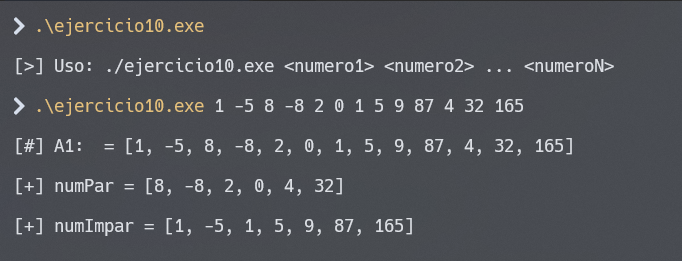
\includegraphics[width=0.8\textwidth,keepaspectratio]{img/ejercicio10.png}
        \end{figure}

%%% REPOSITORIO DE GITHUB %%%

\section{Repositorio de Github}
	\begin{itemize}
		\item Repositorio de Github donde se encuentra el actual laboratorio \\
		\url{https://github.com/ReyserLynnn/ada-lab-b-24b/tree/main/laboratorio01/src}

        \item Repositorio de Github donde se encuentran los laboratorios del curso\\
		\url{https://github.com/ReyserLynnn/ada-lab-b-24b.git}
	\end{itemize}

\clearpage

\section{Cuestionario}
    \begin{enumerate}
        \item \textbf{¿Cómo se declaran los arrays en C++?} \\\\
        En C++, tenemos 2 tipos de arrays: normales y dinámicos. Los arrays normales tienen un tamaño fijo, definido en tiempo de compilación, y se declaran como:
        
            \begin{lstlisting}
int array[10]; 
            \end{lstlisting}
            
            Los arrays dinámicos permiten un tamaño variable en tiempo de ejecución usando punteros y \texttt{new}, y se declaran como:
            \begin{lstlisting}
int* array = new int[size];
            \end{lstlisting}
        
        \item \textbf{Para el siguiente caso: Se desea calcular el total a pagar, en una venta normal en una papelería,
        proporcionando el precio unitario de un producto, así como el número total de productos a comprar,
        además de aplicar el 18\% de IGV. ¿Qué entradas se requiere?¿Cuál es la salida deseada?¿Qué métodos
        produce la salida deseada?} 
            
            \begin{itemize}
                \item \textbf{Entradas requeridas:}
                
                \begin{itemize}
                    \item Precio unitario del producto.
                    \item Número total de productos a comprar.
                \end{itemize}
                
                \item \textbf{Salida deseada:}
                
                \begin{itemize}
                    \item Total a pagar después de aplicar el 18\% de IGV.
                \end{itemize}
                
                \item \textbf{Métodos para producir la salida deseada:}
                
                \begin{itemize}
                    \item Calcular el subtotal: \texttt{subtotal = precio\_unitario * número\_productos}.
                    \item Calcular el IGV (18\%): \texttt{IGV = subtotal * 0.18}.
                    \item Calcular el total a pagar: \texttt{total = subtotal + IGV}.
                \end{itemize}
            \end{itemize}
    \end{enumerate}

\begin{comment}
\section{Referencias}
\begin{itemize}			
	\item \url{https://dialnet.unirioja.es/servlet/articulo?codigo=4573315}
\end{itemize}	    
\end{comment}

\end{document}